\documentclass[landscape]{slides}

\usepackage{amssymb}
\usepackage{alltt}
\usepackage{color}
\usepackage{code}
\usepackage{epsfig}
\usepackage{latexsym}

\definecolor{red}{rgb}{1,0.38,0.000}
\definecolor{darkgreen}{rgb}{0,0.8,0}

\newcommand{\eat}[1]{}

\newcommand{\blue}[1]{{\color{blue}#1}}
\newcommand{\red}[1]{{\color{red}#1}}
\newcommand{\green}[1]{{\color{green}#1}}
\newcommand{\darkgreen}[1]{{\color{darkgreen}#1}}
\newcommand{\yellow}[1]{{\color{yellow}#1}}
\newcommand{\black}[1]{{\color{black}#1}}
\newcommand{\white}[1]{{\color{white}#1}}
\newcommand{\grey}[1]{{\color{grey}#1}}
\newcommand{\mytt}[1]{{\tt #1}}

\newcommand{\ww}{\vspace{-1.5ex}}
\newcommand{\slidetitle}[1]{\red{\Large #1}\vspace{-1ex}}
\newcommand{\subtitle}[1]{\blue{#1}\ww}
\newcommand{\bluett}[1]{\texttt{\blue{#1}}}
\newcommand{\redtt}[1]{\texttt{\red{#1}}}
\newcommand{\bluerm}[1]{\textrm{\blue{#1}}}
\newcommand{\bx}[1]{\black{$#1$}}

\newcommand{\equals}{\blue{$=$}}
\newcommand{\subsumedby}{\blue{$\subseteq$}}
\newcommand{\notsubsumedby}{\blue{$\not\subseteq$}}

\newcommand{\lb}{\texttt{\symbol{123}}}
\newcommand{\rb}{\texttt{\symbol{125}}}
\newcommand{\br}[1]{\lb#1\rb}

\newcommand{\id}[1]{\texttt{#1}}
\newcommand{\bid}[1]{\id{\blue{#1}}}
\newcommand{\blid}[1]{\id{\black{#1}}}
\newcommand{\blit}[1]{\black{\emph{#1}}}

\newcommand{\eone}{$e_1$}
\newcommand{\etwo}{$e_2$}
\newcommand{\ethree}{$e_3$}
\newcommand{\vone}{$v_1$}
\newcommand{\vtwo}{$v_2$}
\newcommand{\evar}{$e$}
\newcommand{\vvar}{$v$}
\newcommand{\avar}{$a$}
\newcommand{\dvar}{$d$}

\newcommand{\var}[1]{\id{{\$}$#1$}}
\newcommand{\set}[1]{\{#1\}}
\newcommand{\att}[2]{\id{attribute $#1$ \br{ $#2$ }}}
\newcommand{\comatt}[2]{\id{attribute \br{ $#1$ } \br{ $#2$ }}}
\newcommand{\elt}[2]{\id{element $#1$ \br{ $#2$ }}}
\newcommand{\comelt}[2]{\id{element \br{ $#1$ } \br{ $#2$ }}}
\newcommand{\seq}{\mathbin{\id{,}}}
\newcommand{\choice}{\mathbin{\id{|}}}
\newcommand{\emp}{\id{()}}

\newcommand{\dsh}{\id{-}}
\newcommand{\str}{\id{*}}
\newcommand{\opt}{\id{?}}
\newcommand{\pls}{\id{+}}

\newcommand{\Primes}[1]{\mbox{P$'$($#1$)}}
\newcommand{\Prime}[1]{\mbox{P($#1$)}}
\newcommand{\Quant}[1]{\mbox{Q($#1$)}}

\newcommand{\at}{\id{@}}
\renewcommand{\slash}{\mathbin{\id{/}}}
\newcommand{\slashslash}{\mathbin{\id{//}}}
\newcommand{\brackets}[1]{\id{[$#1$]}}

\newcommand{\subst}[2]{\id{\{$\var{#1}$ := $#2$\}}}
\newcommand{\forloop}[3]{\id{for $\var{#1}$ in $#2$ return $#3$}}
\newcommand{\paren}[1]{\id{($#1$)}}

\newcommand{\Nextline}{\\ \\ \\}

\newenvironment{Slide}[1]{\begin{slide}\slidetitle{#1}}{\vfill\end{slide}}

\newenvironment{TitleSlide}[2]{\begin{slide}
\begin{center}\LARGE\color{red}#1\large\color{blue}#2}{\end{center}
\end{slide}}

\newcounter{partctr}
\renewcommand{\thepartctr}{\Roman{partctr}}
\newcounter{subpartctr}[partctr]
\renewcommand{\thesubpartctr}{\Roman{partctr}.\arabic{subpartctr}}

\newcommand{\partslide}[1]{
 \begin{slide}
 \begin{center}\Large\color{blue}
 \refstepcounter{partctr}
 Part \thepartctr\\[2ex]\LARGE\color{red}
 #1
 \end{center}
 \end{slide}
}

\newcommand{\prologslide}[1]{
 \begin{slide}
 \begin{center}\Large\color{blue}
 Prolog\\[2ex]\LARGE\color{red}
 #1
 \end{center}
 \end{slide}
}

\newcommand{\preludeslide}[1]{
 \begin{slide}
 \begin{center}\Large\color{blue}
 Prelude\\[2ex]\LARGE\color{red}
 #1
 \end{center}
 \end{slide}
}

\newcommand{\interludeslide}[1]{
 \begin{slide}
 \begin{center}\Large\color{blue}
 Interlude\\[2ex]\LARGE\color{red}
 #1
 \end{center}
 \end{slide}
}

\newcommand{\epilogslide}[1]{
 \begin{slide}
 \begin{center}\Large\color{blue}
 Epilog\\[2ex]\LARGE\color{red}
 #1
 \end{center}
 \end{slide}
}

\newcommand{\subpartslide}[1]{
 \begin{slide}
 \begin{center}\Large\color{blue}
 \refstepcounter{subpartctr}
 Part \thesubpartctr\\[2ex]\LARGE\color{red}
 #1
 \end{center}
 \end{slide}
}

\newcommand{\quoteslide}[2]{
 \begin{slide}
 \begin{quote}
 \blue{#1}
 \begin{flushright}
 \red{--- #2}
 \end{flushright}
 \end{quote}
 \end{slide}
}

\newenvironment{tightitemize}{
  \begin{list}{$\bullet$}{
    \setlength{\topsep}{0ex}
    \setlength{\itemsep}{1ex}
    \setlength{\parsep}{0ex}
    \setlength{\partopsep}{0ex}
  }
}{
  \end{list}
}

\newenvironment{tighteritemize}{
  \begin{list}{$\bullet$}{
    \setlength{\topsep}{0ex}
    \setlength{\itemsep}{0ex}
    \setlength{\parsep}{0ex}
    \setlength{\partopsep}{0ex}
  }
}{
  \end{list}
}

\newcommand{\bluetriangle}[0]{{\blue{$\blacktriangleright$}}}
\newcommand{\whitetriangle}[0]{{\white{$\blacktriangleright$}}}
\newcommand{\greentriangle}[0]{{\green{$\blacktriangleright$}}}
\newcommand{\redtriangle}[0]{{\red{$\blacktriangleright$}}}

\newcommand{\lbluetriangle}[0]{{\blue{$\blacktriangleleft$}}}
\newcommand{\lgreentriangle}[0]{{\green{$\blacktriangleleft$}}}
\newcommand{\lredtriangle}[0]{{\red{$\blacktriangleleft$}}}

\newcommand{\vl}{\vspace*{0.5cm}}
\newcommand{\vv}{\vspace*{1cm}}
\newcommand{\hh}{\hspace*{0.5cm}}
\newcommand{\hhh}{\hspace*{0.8cm}}

\newcommand{\bb}{\redtriangle\ }
\newcommand{\dbb}{\redtriangle\redtriangle\ }
\newcommand{\bbb}{\hhh\bluetriangle\ }
\newcommand{\bbw}{\hhh\whitetriangle\ }
\newcommand{\bbbb}{\hhh\hhh\greentriangle\ }

\newcommand{\lbb}{\lredtriangle}
\newcommand{\ldbb}{\ \lredtriangle\lredtriangle}

\newcommand{\redbr}[1]{\red{\lb}#1\red{\rb}}
\newcommand{\arrow}{\Rightarrow}

\sloppy \setlength{\topmargin}{0in} \addtolength{\topmargin}{-1.0in}
\addtolength{\textheight}{1.5in}



\newcommand{\scream}[1]{\textbf{#1}}

\newcommand{\notes}[1]{{\tiny #1}}
%\newcommand{\notes}[1]{}

\newcounter{chap}
\stepcounter{chap}

%%%%%%%%%%%%%%%%%%%%%%%%%%%%%%%%%%%%%%%%%%%%%%%%%%%%%%%%%%%%%%%%%%%%%%%%
\begin{document}
%%%%%%%%%%%%%%%%%%%%%%%%%%%%%%%%%%%%%%%%%%%%%%%%%%%%%%%%%%%%%%%%%%%%%%%%

% Title slide
\begin{slide}
\begin{center}\Large\color{blue}
PADX\\Enabling XQuery over Ad-hoc Data Sources

\large\color{black}
\begin{center}
Mary Fern\'andez, AT\&T Labs Research\\
Kathleen Fisher, AT\&T Labs Research\\
Bob Gruber, Google Inc.\\
Yitzhak Mandelbaum, Princeton University
\end{center}
\end{center}
\end{slide}

\begin{Slide}{Existing Technologies}
  
  \vspace*{1cm}
  \bb PADS\\
  \bbb Declarative data-stream description language\\
  \bbb Syntax \& semantics of \emph{\blue{semi-structured}}, ad hoc data sources \\
  \bbb From description, compiler generates\\
  \bbbb Parsing library with error detection \& recovery\\
  \bbbb In-memory representation of data

  \bb XQuery\\
  \bbb Functional, strongly typed XML query language \\
  \bbb Well-suited to querying \emph{\blue{semi-structured}} sources

  \bb Galax\\
  \bbb Complete, extensible, efficient implementation of XQuery

\end{Slide}

\begin{Slide}{Describing HTTP Common Log Format}

  \bb Example HTTP CLF Data

{\small
\begin{alltt}
\blue{100.222.33.44 - - [15/Oct/1997:18:46:51 -0700] "GET /foo/bar.txt HTTP/1.0" 200 30}
\end{alltt}
}
  \bb PADS Description

{\small
\begin{alltt}
Pstruct http_clf_t \{
        clihost_t \textbf{host};              /- IP address of client requesting service
   ' '; auth_id_t \textbf{remoteID};          /- Remote identity; '-' means not obtained
   ' '; auth_id_t \textbf{auth};              /- Name of authenticated user
   " [";
   Pdate(:']':) \textbf{my_date};             /- Timestamp of request
   "] ";
   http_request_t \textbf{request};           /- Request
   ' ';  Puint16_FW(:3:) \textbf{response};   /- 3-digit response code
   ' ';  contentOpt_t \textbf{contentLength}; /- Number of bytes in request response
\};
\end{alltt}}

\bb Parsing library called from host application

{\small
\begin{alltt}
  http_clf_t http_clf;        /* In-memory representation */
                              /* Read procedures */  
  Perror_t http_clf_t_read(..., &http_clf, ...); 
\end{alltt}}


\end{Slide}

\begin{Slide}{Viewing \& Querying HTTP CLF}

  \bb Virtual XML view 
{\small
\begin{alltt}
\blue{<http-clf>
  <\textbf{host}>100.222.33.44</host>
  <\textbf{remoteID}><unauthorized/></remoteID>
  <auth><unauthorized/></auth>
  <mydate>15/Oct/1997:18:46:51 -0700</mydate>
  <request>
    <meth>GET</meth>
    <req_uri>/foo/bar.txt</req_uri>
    <version><major>1</major><minor>0</minor></version>
  <response>200</response>
  <contentLength>30</contentLength>
<http-clf>}
\end{alltt}
}

\bb Using XQuery to explore data\\
\bbb Hosts of records with content length greater than 2K

{\small
\begin{alltt}
\blue{./PSource/http-clf[contentLength > 2048]/host}
\end{alltt}}

\bbb Locations of records with error in content-length field

{\small
\begin{alltt}
\blue{./PSource/http-clf[contentLength/pd/errCode]/pd/loc}
\end{alltt}}
\end{Slide}

\begin{Slide}{PADX Architecture} 
  \centerline{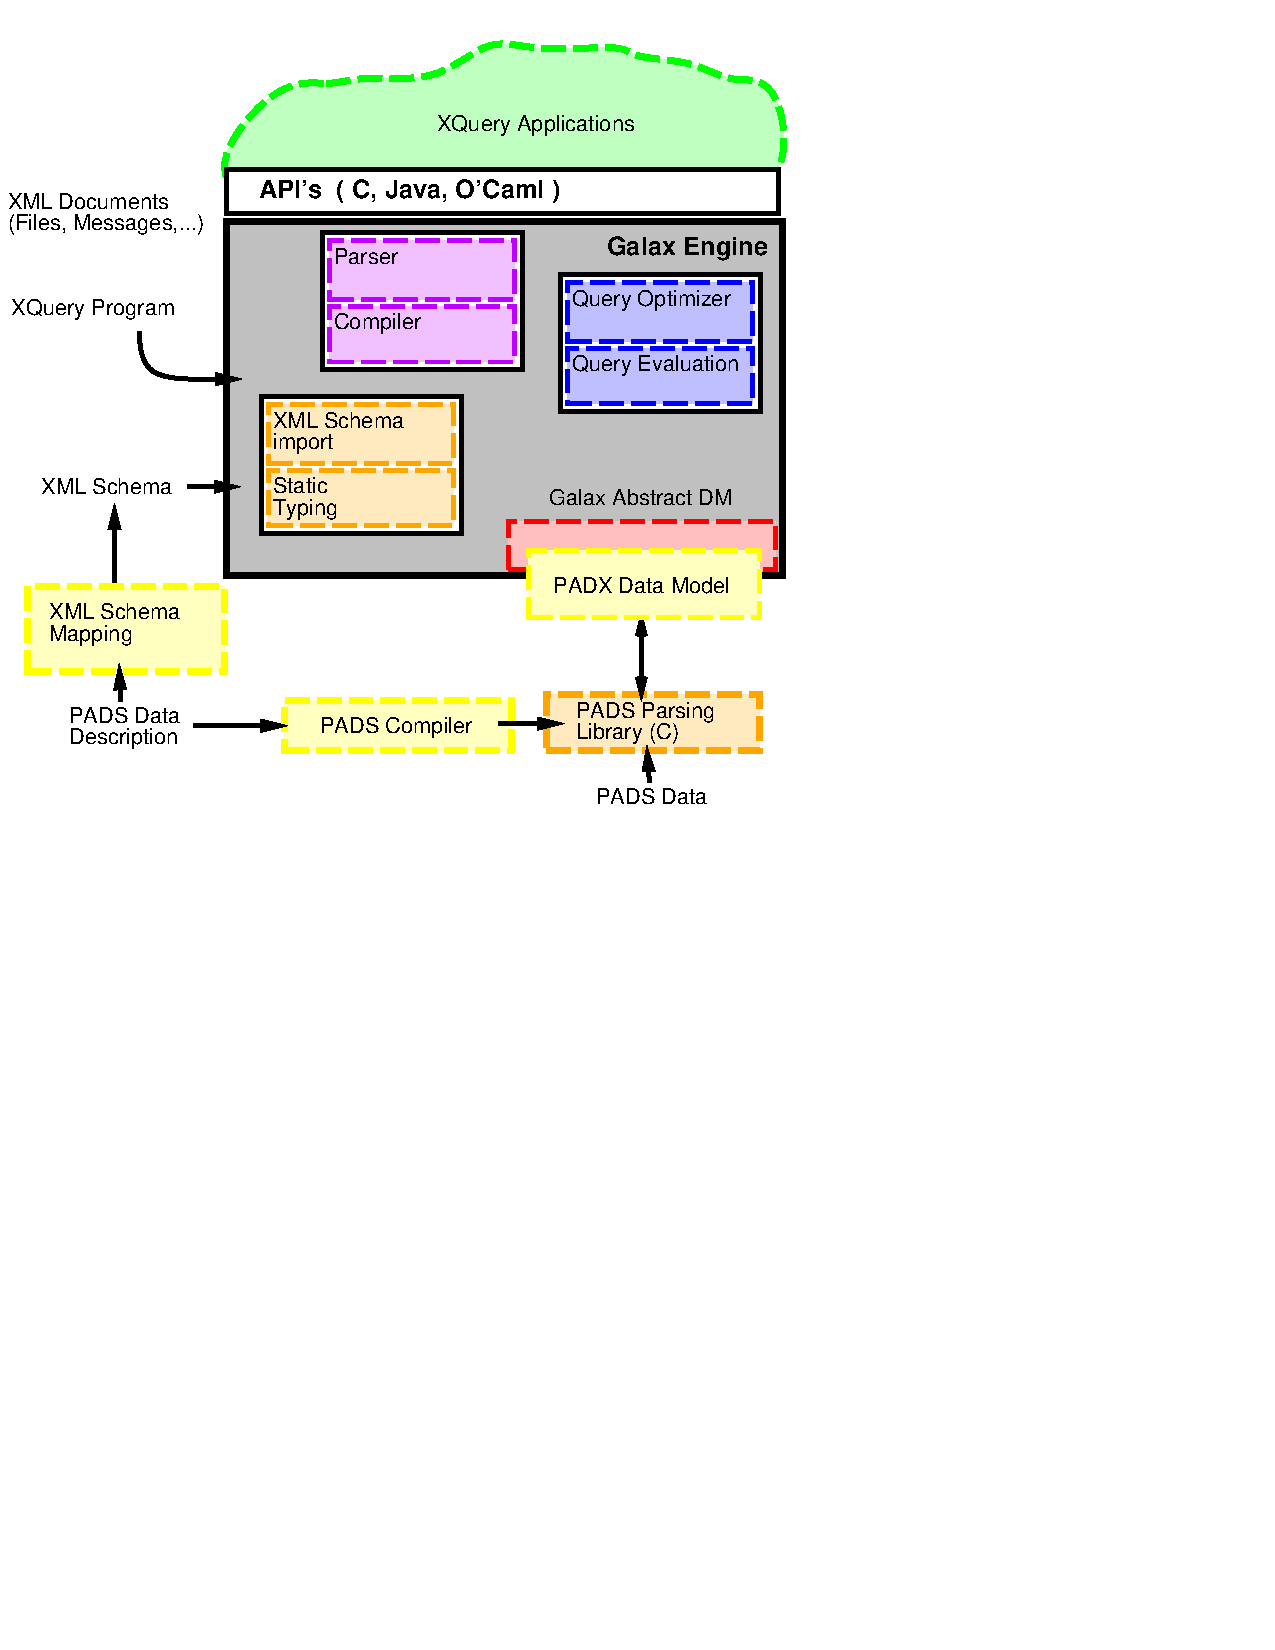
\psfig{file=pads-galax-overview-yitzhak.pdf}}
\end{Slide}

\begin{Slide}{Technical Challenges}

  \bb Natural mapping from PADS description to XML Schema 

  \bb Materialize PADS data as virtual XML \\
  \bbb Implement Galax's abstract tree data model on top of PADS 

  \bb Memory management of PADS records \\
  \bbb Data exceeding memory limits requires clever MM\\
  \bbb PADS program typically reads records sequentially \\
  \bbb Galax may not access records sequentially \\
  \bbb Harkens back to MM in object-oriented databases

  \bb User-friendly interface\\
  \bbb Describe PADS data, compile library, write \& execute queries
\end{Slide}

\begin{Slide}{Project Status}

\bb PADS

\bb Galax

\bb PADX

\bb Integration effort successful 

\bb More thorough regression testing

\bb Demonstrate to potential users

\bb Research problems\\
\bbb Extending Galax's data model to leverage streams access\\
\bbb More efficient meta-data structures in PADS 

\end{Slide}

\begin{Slide}{Abstract Tree Data Model}
\vspace*{1cm}
\bb Fragment of Galax's abstract tree data model\\
\bbb Full navigation of XML tree\\
\bbb Access to atomic values

{\small
\begin{alltt}
  method virtual \blue{node_name}    : unit -> atomicQName option

  method virtual \blue{typed_value}  : unit -> atomicValue cursor

  method virtual \blue{parent}       : unit -> node option
  method virtual \blue{children}     : unit -> \green{node cursor}

  method virtual \blue{docorder}  : unit -> Nodeid.docorder
\end{alltt}}

\bb Cursor : lazy iterator access to node sequence\\
\bb Node identity \& document order : canonical order 

\end{Slide}

\begin{Slide}{Accessing Record Sequences}

  \bb Access to record (node) sequence \\
  \bbb Read all items in sequence \\
  \bbb Produce items on demand

  \bb Each record field materialized strictly as needed

  \bb Solution: \\
  \bbb Choose record as read granularity \\
  \bbb Read record on demand \\
  \bbb Maintain meta-data for fast re-retrieval
\end{Slide}

%%%%%%%%%%%%%%%%%%%%%%%%%%%%%%%%%%%%%%%%%%%%%%%%%%%%%%%%%%%%%%%%%%%%%%%%
\end{document}
%%%%%%%%%%%%%%%%%%%%%%%%%%%%%%%%%%%%%%%%%%%%%%%%%%%%%%%%%%%%%%%%%%%%%%%%

